\section{Enhanced Weathering}
The lifecycle of enhanced rock weathering consists of three stages: 1. The mining and processing stage, 2. the transport and application stage, and 3. the weathering and dissolution stage. The first two stages lead from the rock in a mine to the application of the rock dust on the field and usually cause significant carbon emissions, while the final stage, which spans years to decades, contributes the negative emissions by drawing carbon dioxide from the air during weathering.
\subsection{Mining and processing}
\subsection{Transport and application}
\subsection{Weathering}
\subsection{Calculation of steady-state olivine weathering rate and levelized cost}
\subsubsection{Weathering rate and dissolution time}
In the first step, calculating the weathering rate and total dissolution time of olivine rock, depending on the soil acidity and temperature is necessary.\vspace{2mm}

Weathering rates for olivine-rich rock material, dependent on soil pH values, are available from the literature, based on a range of experiments conducted at a constant temperature of 25 °C (See Fig. 2.1).
\begin{figure}[h]
  \begin{center}
    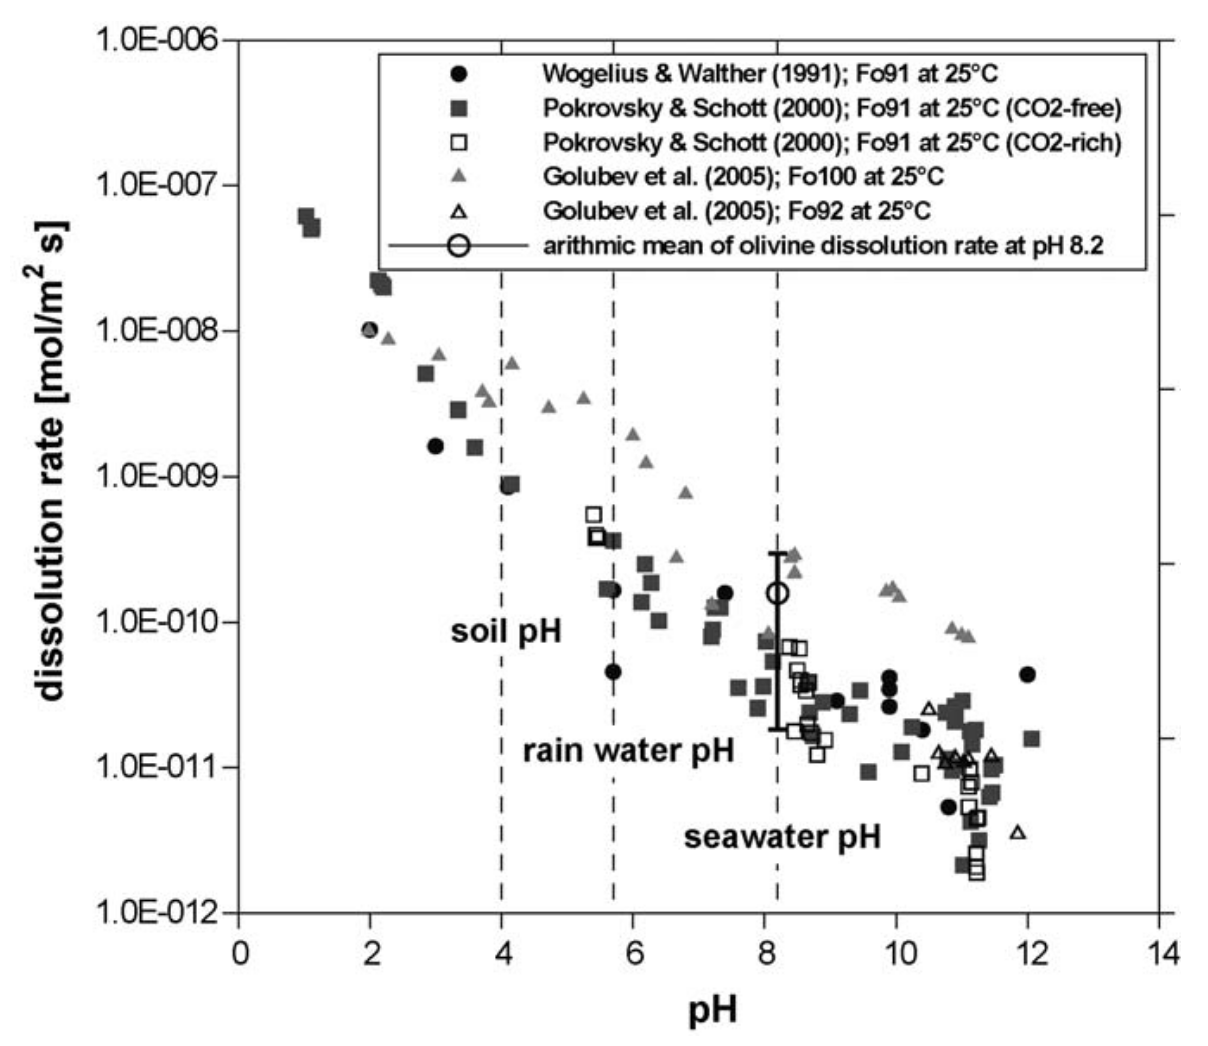
\includegraphics[width=0.5\textwidth]{figures/ewr_1.png}
    \caption{Olivine dissolution rate \(R_{{\text{diss}}}\) in mol/m$^2$s dependent on soil pH values \parencite{hangx_coastal_2009}}
    \label{fig:figure2}
  \end{center}
\end{figure}\hfill \break
From these datapoints, a logarithmic relationship was extrapolated:
\begin{equation}
  \log_{10}{R_{{\text{diss}}, 25}(pH)} = -7.3656 - 0.297 * pH
\end{equation}
In order to adjust the weathering rate for the environmental temperature, the Arrhenius-relationship based formula derived by \textcite{wogelius_olivine_1992} was rearranged \footnote{For the derivation of formulas 3.2 and 3.6, see Appendix} to
\begin{equation}
  \log_{10}{R_{\text{diss}}(pH, K)} = 1.972R*\left(\frac{1}{262.15}-\frac{1}{K}\right)+\log_{10}{R_{{\text{diss}}, 25}(pH)}
\end{equation}
with the target temperature \(K\), given in Kelvin, and the gas constant \(R\) (\(8.3145 J \frac{mol}{K}\)).
The shrinking core dissolution model developed by \textcite{hangx_coastal_2009} can then be used to calculate the dissolved fraction of material after time:
\begin{equation}
  X(t) = 1-\frac{d(t)^3}{d_0^3} = \frac{d_0^3-(d_0-2R_{\text{diss}}\Omega t)^3}{d_0^3}
\end{equation}
where \(d_0\) is the beginning grain size in meters, \(\Omega\) is the molar volume of the input material, and \(t\) is the elapsed time in seconds. Rearranged for \(t\), this formula can be used to calculate the time until dissolution
\begin{equation}
  t = \frac{d_0[1-(1-\frac{X}{100})^\frac{1}{3}]}{2R_{\text{diss}}\Omega}
\end{equation}
with \(X\) being the desired dissolution grade in percent.\vspace{2mm}

\subsubsection{Effective annual dissolution rate}
In the second step, the required annual application rate per hectare to reach a steady state of application and dissolution has to be calculated.
Let the remaining fraction of the initial rock mass at time \(t\) be \(m(t) = 1 - X(t) = \frac{d(t)^3}{d_0^3}\). Since the final dissolution time \(T=\frac{d_0}{2R_{\text{diss}}\Omega}\), this can also be written as
\begin{equation}
  m(t) = \left(1 - \frac{t}{T}\right)^3
  \quad\text{for } 0 \le t \le T
\end{equation}
Now, let \(L\) be the average lifetime of the rock material, and \(y\) the number of years since the beginning of the reaction, such that\footnotemark[1]
\begin{equation}
  L = \int_0^{\infty}m(y)\,dy= \int_0^Y\left(1-\frac{y}{Y}\right)^3\,dy = \frac{Y}{4}
\end{equation}
In order to calculate the yearly dissolution rate of the rock material, the remaining mass fraction can be approximated by the exponential decay function
\begin{equation}
  m(y) = e^{-ky}
\end{equation}
for which the average lifetime \(L\) can be calculated using
\begin{equation}
  L = \int_0^\infty e^{-ky} dy = \frac{1}{k}
\end{equation}
which, by plugging in the result of (3.6), can be rearranged to
\begin{equation}
  k = \frac{1}{L} = \frac{4}{Y}
\end{equation}
Finally, the annual effective dissolution rate \(f_{\text{eff}}\) can be calculated using
\begin{equation}
  f_{\text{eff}} = 1-e^{-k}=1-e^{-\frac{4}{Y}}
\end{equation}
\subsubsection{Steady-state results}
For a given area of land, say one hectare, the inventory of rock material \(S_t\) at the beginning of a period \(t\) is equal to the inventory of the previous period \(S_{t-1}\), less the dissolved material \(D_{t-1} = S_{t-1}*f_{\text{eff}}\), plus any addition \(A_{t-1}\), with additions assumed to occur at the end of each period.\vspace{2mm}

In a steady-state scenario, the amount of rock spread annually would exactly equal the amount of rock dissolved in the same timeframe, such that
\begin{equation}
  S^* = \frac{A^*}{f_{\text{eff}}}
\end{equation}
By rearranging for \(A^*\), this allows for the calculation of the required annual addition in order to achieve and maintain a desired steady-state rock inventory of \(S^*\):
\begin{equation}
  A^* = S^* * f_{\text{eff}}
\end{equation}

\subsubsection{Calculation of LCOC}
The levelized cost of carbon including transport (LCOCR) is then calculated as the total cost of the project over its $T = 100$ year lifetime divided by the total amount of CO2 removed in the same timeframe:
\begin{equation}
  \text{LCOCR} = \frac{C_r \sum_{t=1}^{T} A_t}{\eta \sum_{t=1}^{T} D_t} = \frac{C_r T A^*}{\eta \sum_{t=1}^{T} D_t} = \frac{C_rT}{\eta\left(T-\frac{1-(1-f_{\text{eff}})^T}{f_{\text{eff}}}\right)}
\end{equation}
where \(C_r\) is the total cost of one tonne of rock material, defined as the sum of CapEx, fixed cost and variable cost per tonne, and \(\eta\) is the amount of CO2 absorbed by one tonne of rock until complete dissolution (\(\eta = 0.76\) for olivine rock of 60\% purity).
Note that the total amount of rock dissolved is not equal to the total amount of rock applied, since the amount dissolved per year is lower during the "ramp-up" phase until the steady state is reached, and the steady state inventory of \(S^*\) remains on the field after the end of the project timeline.\vspace{2mm}

To calculate the levelized cost of carbon considering transport and leakage \(\text{LCOCR}^+\), the leakage rate \(\alpha\), which is calculated from the amount of CO2 emitted during mining, transport, and application, is applied to the LCOCR:
\begin{equation}
  \text{LCOCR}^+ = \frac{\text{LCOCR}}{1-\alpha}
\end{equation}

\subsection{Case Study: Enhanced rock weathering in the USA}
The United States can serve as a useful case study for enhanced rock weathering due to its large land area and high technological and economic development.\vspace{2mm}

The primary input variables for the present enhanced weathering model are energy and labour costs, the environmental conditions (i.e. the average pH value and temperature of the soil), the chosen grain size of the rock dust (\(d_0\)), as well as the desired steady-state inventory per hectare (\(S^*\)). For the full overview of input variables for the US-base example case, see tables 3.1 and 3.2.\vspace{2mm}

The data on global average soil temperatures and pH values was collected from \textcite{lembrechts_global_2022} and \textcite{hengl_soilgrids250m_2017}, respectively, and processed using the open-source QGIS application.\hfill
\begin{figure}[ht]
  \centering
  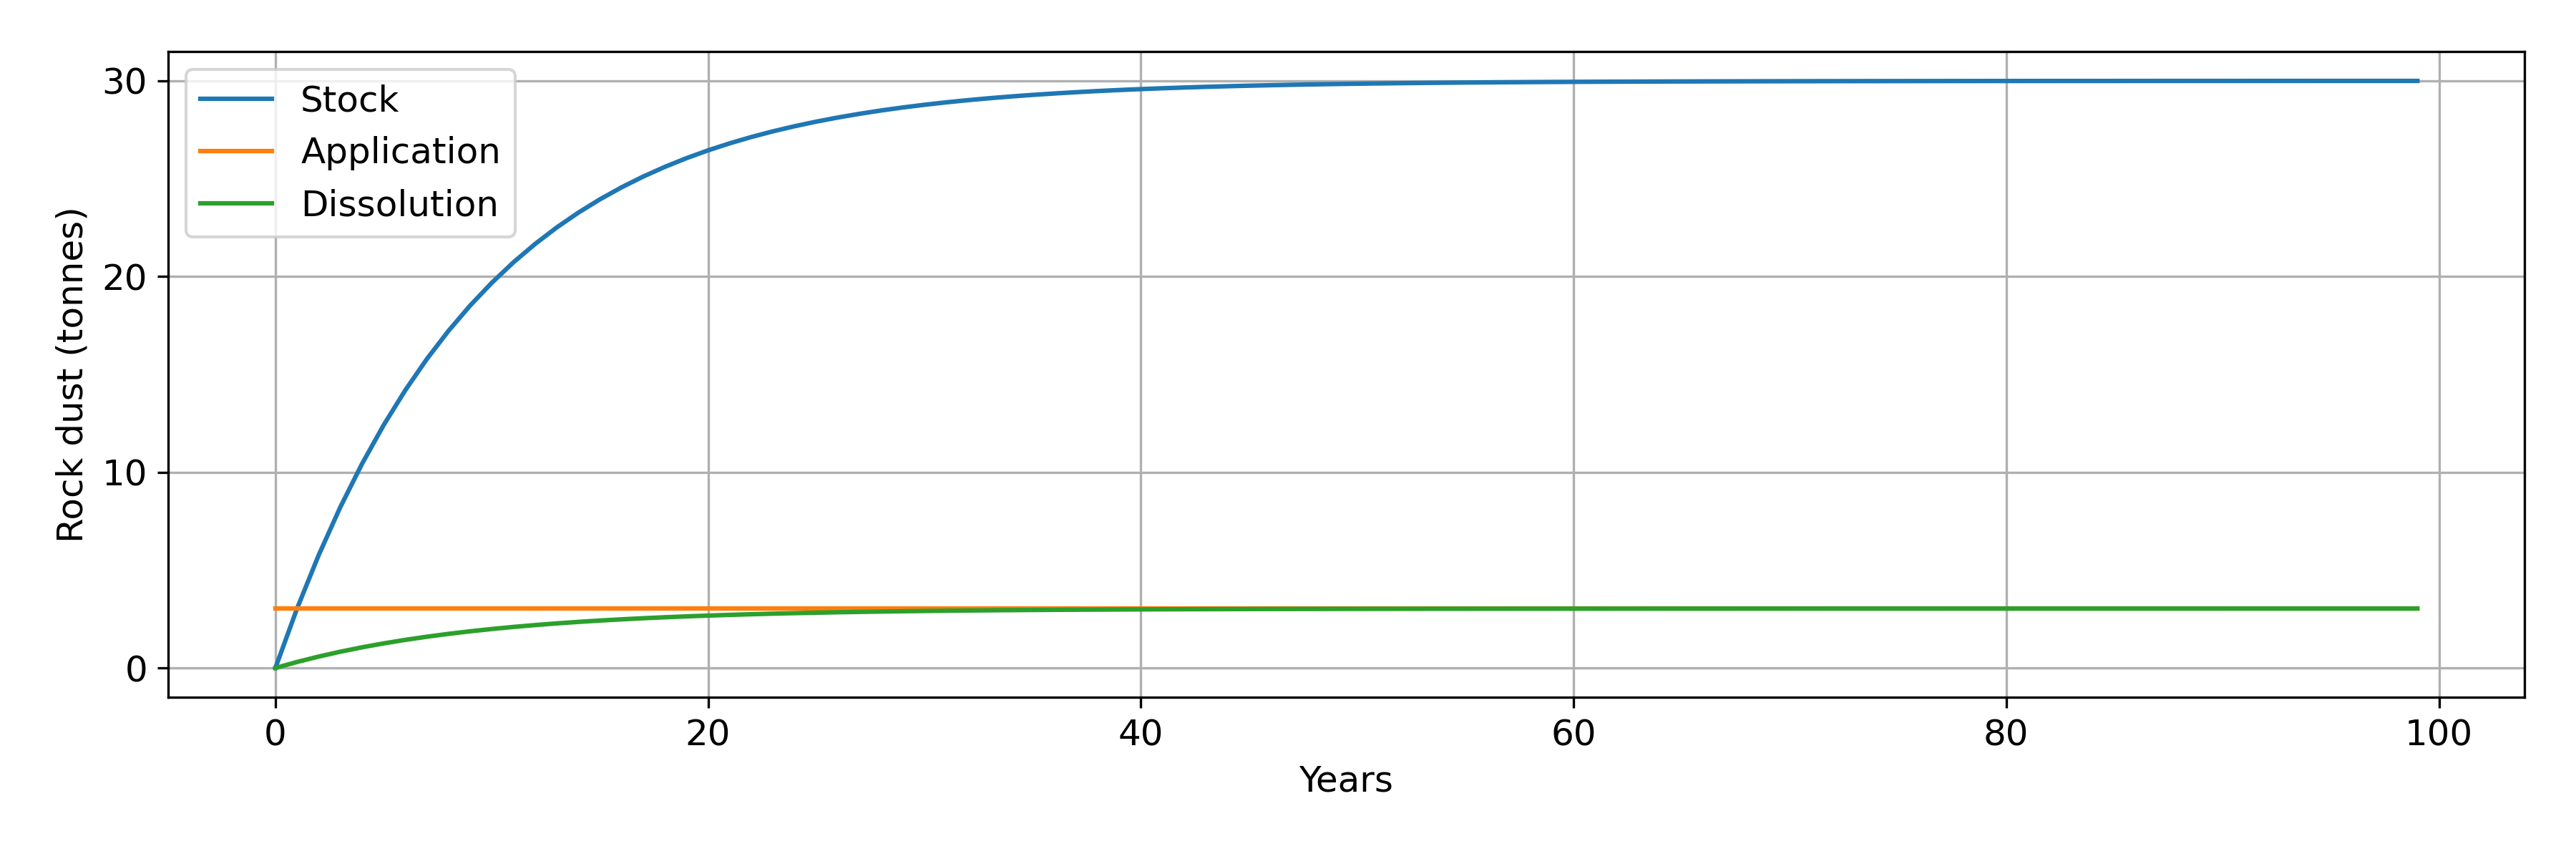
\includegraphics[width=1\linewidth]{figures/EW_usa_case.png}
  \caption{Timeline of an example 100 year EWR project in the United States}
  \label{fig:usa_sample_case}
\end{figure}
\begin{wraptable}{r}{9.5cm}
\vspace*{-\baselineskip}
  \begin{tabular}{lll}
    \textbf{General economic variables}                          &                                   & \multicolumn{1}{r}{}        \\ \hline
    \multicolumn{1}{|l|}{Capital recovery factor}      & \multicolumn{1}{l|}{\%}           & \multicolumn{1}{r|}{9.44} \\ \hline
    \multicolumn{1}{|l|}{Electricity price}            & \multicolumn{1}{l|}{\$ / MWh}     & \multicolumn{1}{r|}{44.00}  \\ \hline
    \multicolumn{1}{|l|}{Electricity carbon intensity} & \multicolumn{1}{l|}{g / kWh}      & \multicolumn{1}{r|}{400}    \\ \hline
    \multicolumn{1}{|l|}{Diesel price}                 & \multicolumn{1}{l|}{\$ / L}             & \multicolumn{1}{r|}{0.9}    \\ \hline
    \multicolumn{1}{|l|}{Diesel carbon intensity}      & \multicolumn{1}{l|}{g / km}       & \multicolumn{1}{r|}{250}    \\ \hline
    \multicolumn{1}{|l|}{Diesel carbon intensity}      & \multicolumn{1}{l|}{kg / l}       & \multicolumn{1}{r|}{2.7}    \\ \hline
    \multicolumn{1}{|l|}{Avg. cost per worker-hour}    & \multicolumn{1}{l|}{\$ / hour}    & \multicolumn{1}{r|}{70.05}  \\ \hline
    \multicolumn{1}{|l|}{Truckload tonnage}            & \multicolumn{1}{l|}{t}            & \multicolumn{1}{r|}{40.00}  \\ \hline
    \multicolumn{1}{|l|}{Truck fuel consumption}       & \multicolumn{1}{l|}{l / km}       & \multicolumn{1}{r|}{0.40}   \\ \hline
    \multicolumn{1}{|l|}{Truck avg. speed}             & \multicolumn{1}{l|}{km / hr}      & \multicolumn{1}{r|}{80}     \\ \hline
    \multicolumn{1}{|l|}{Rail energy consumption}      & \multicolumn{1}{l|}{kWh / tkm} & \multicolumn{1}{r|}{0.1836} \\ \hline
    \multicolumn{1}{|l|}{Tractor fuel consumption}     & \multicolumn{1}{l|}{l / h}        & \multicolumn{1}{r|}{16}     \\ \hline
        &                                &                                  \\
    \textbf{EWR-specific variables}                       &                                   &                             \\ \hline
    \multicolumn{1}{|l|}{Desired  \(S^*\)}           & \multicolumn{1}{l|}{t / ha}       & \multicolumn{1}{r|}{30}     \\ \hline
    \multicolumn{1}{|l|}{Particle size \(d_0\)}                & \multicolumn{1}{l|}{micron}       & \multicolumn{1}{r|}{10}     \\ \hline
    \multicolumn{1}{|l|}{Avg. soil pH value}                & \multicolumn{1}{l|}{}       & \multicolumn{1}{r|}{6.229}     \\ \hline
    \multicolumn{1}{|l|}{Avg. soil temperature}                & \multicolumn{1}{l|}{°C}       & \multicolumn{1}{r|}{8.961}     \\ \hline
  \end{tabular}
  \captionof{table}{ERW input variables, US-based case}\label{us-case-table}
\end{wraptable}
Based on these inputs, and using formulas (3.1) and (3.2), the average dissolution rate for the United States was calculated to be \(R_\text{diss, USA} = 9.83494 * 10^{-11} \frac{mol}{sec}\). This results in a final dissolution time of \(T_\text{USA} = 37.47\) years, with the average lifetime of \(L_\text{USA} = 9.37\) years, and the effective annual dissolution rate \(f_\text{eff, USA} = 10.12\%\). This rate means that an annual application of \(A^* = \frac{30}{0.1012} = 3.04 \frac{tonnes}{ha}\) is required to eventually reach a steady state inventory of \(S^* = 30 \frac{tonnes}{ha}\) after approximately 90 years, with 95\% of the progress being achieved within the first 35 years (see Figure 3.2). In the steady state, the annual dissolution (\(D_t\)) will equal the application (\(A^*\)), and the carbon dioxide removed annually in this example case can be calculated as \(CDR(t) = \eta D_t = 0.76\frac{t \ CO^2}{t \ OL}*3.04\frac{t \ OL}{ha}\ = 2.3104 \frac{t \ CO^2}{ha}\).\vspace{2mm}

To calculate the cost per tonne of rock material applied, a sample mining operation with a volume of 15 Mt rock per year is used. This yields CapEx of 0.63 US\$ and, assuming annual maintenance costs of 2.2\% of total CapEx, fixed costs of 0.147 US\$, per tonne of olivine rock applied to the field. Furthermore, the variable cost is calculated from the energy and labour required for processing, transport and application, and adds 33.51 US\$ per tonne.\footnote{For the detailed calculations, see Appendix ..} This shows that the majority of the cost is attributable to the labour and logistics required for processing and application, while CapEx and fixed costs make up only a small fraction of the total costs.\vspace{2mm}

Plugging in the cost per tonne of rock material applied into formula (3.13) yields a LCOCR of 50.07 US\$ per tonne of CO$_2$ removed. Finally, the leakage factor $\alpha$ is calculated to be 18.66\%, based on the amount of electric energy and Diesel used in the entire process and their respective emission factors from table 3.1. Using formula (3.14), this results in a final LCOCR$^+$ of 61.55 US\$.
